\chapter{Prototype 1}
\label{ch:prototype1}
In this chapter we explain the role activPal plays in our prototype and we discuss the paper sketches that were a result of a brainstorming session conducted by the authors. In addition the running prototype and the technology and frameworks used to create it are presented.

\section{activPAL}
As mentioned in Section~\ref{sensorActivPal} the activPAL classifies the accelerometer data into 3 different types of behaviour, this data can then be viewed through activPALs proprietary software. There is an alternative to export the data in a \gls{csv} format, and there are several options as how the data should be presented or aggregated. 

It is possible to display raw accelerometer data or provide event based data where a new entry is created if the state has changed. A new line will then be written with the time, duration and state type every time the state changes. A more detailed overview of the \gls{csv} file can be found in Appendix~\ref{csvDocument}.

For the purpose of our thesis the event based \gls{csv} was the most suited format for the type of information we would need to create visualizations. Before feeding the data to our visualizations the system parses the data into more suitable data structures. activPAL is not a key part of our prototype, we chose this sensor because it had been proven trustworthy in other research, and was easy to acquire. Other sensor can be used as long as the data has the correct data format.

% REVIEW, I NEED IT.
\section{Paper Sketches}
\label{sec:paperSketches}
Before starting the implementation of the system we created a set of paper sketches of the visualizations that we planned to implement. These were our first ideas on the visualizations that would fulfil the initial requirements efficiently, while providing several alternatives to choose from.

\subsection{Overview charts}
Getting an overview of the week as a whole can be useful as an introduction. By looking at an overview the user can quickly identify bad days that can then be investigated further. In other words these visualizations address the weekly overview requirement IR-1. They can also be used as the top level of an interactive application. Each day could then be clicked to show either a timeline or pie chart.

The overview charts mainly focus on two type of visual variables (as described in Section~\ref{sec:visualVarables}): Position and size. If we look at Figure~\ref{fig:smileyWeek}, we see that the horizontal position of elements is used to illustrate how the day was classified. The close proximity of the elements in each horizontal level, makes us intuitively associate days that are on the same level as being part of a group. The size of each group makes it easy to see which classification has the most amount of days. Since size has a quantitative characteristic we can easily see that the top classification has twice as many days as the middle one, and four times as many as the bottom one.

\subsubsection{Day classification}
By calculating the overall activity level and classifying the days into three categories the physiotherapist can easily see which days a patient needs to be more active and which days the activity level is satisfactory. In our sketch, (see Figure \ref{fig:smileyWeek}, the three different classifications are illustrated by smilies (smiling face for active days, and sad face for inactive days).

\begin{figure}[h!]
	\centering
		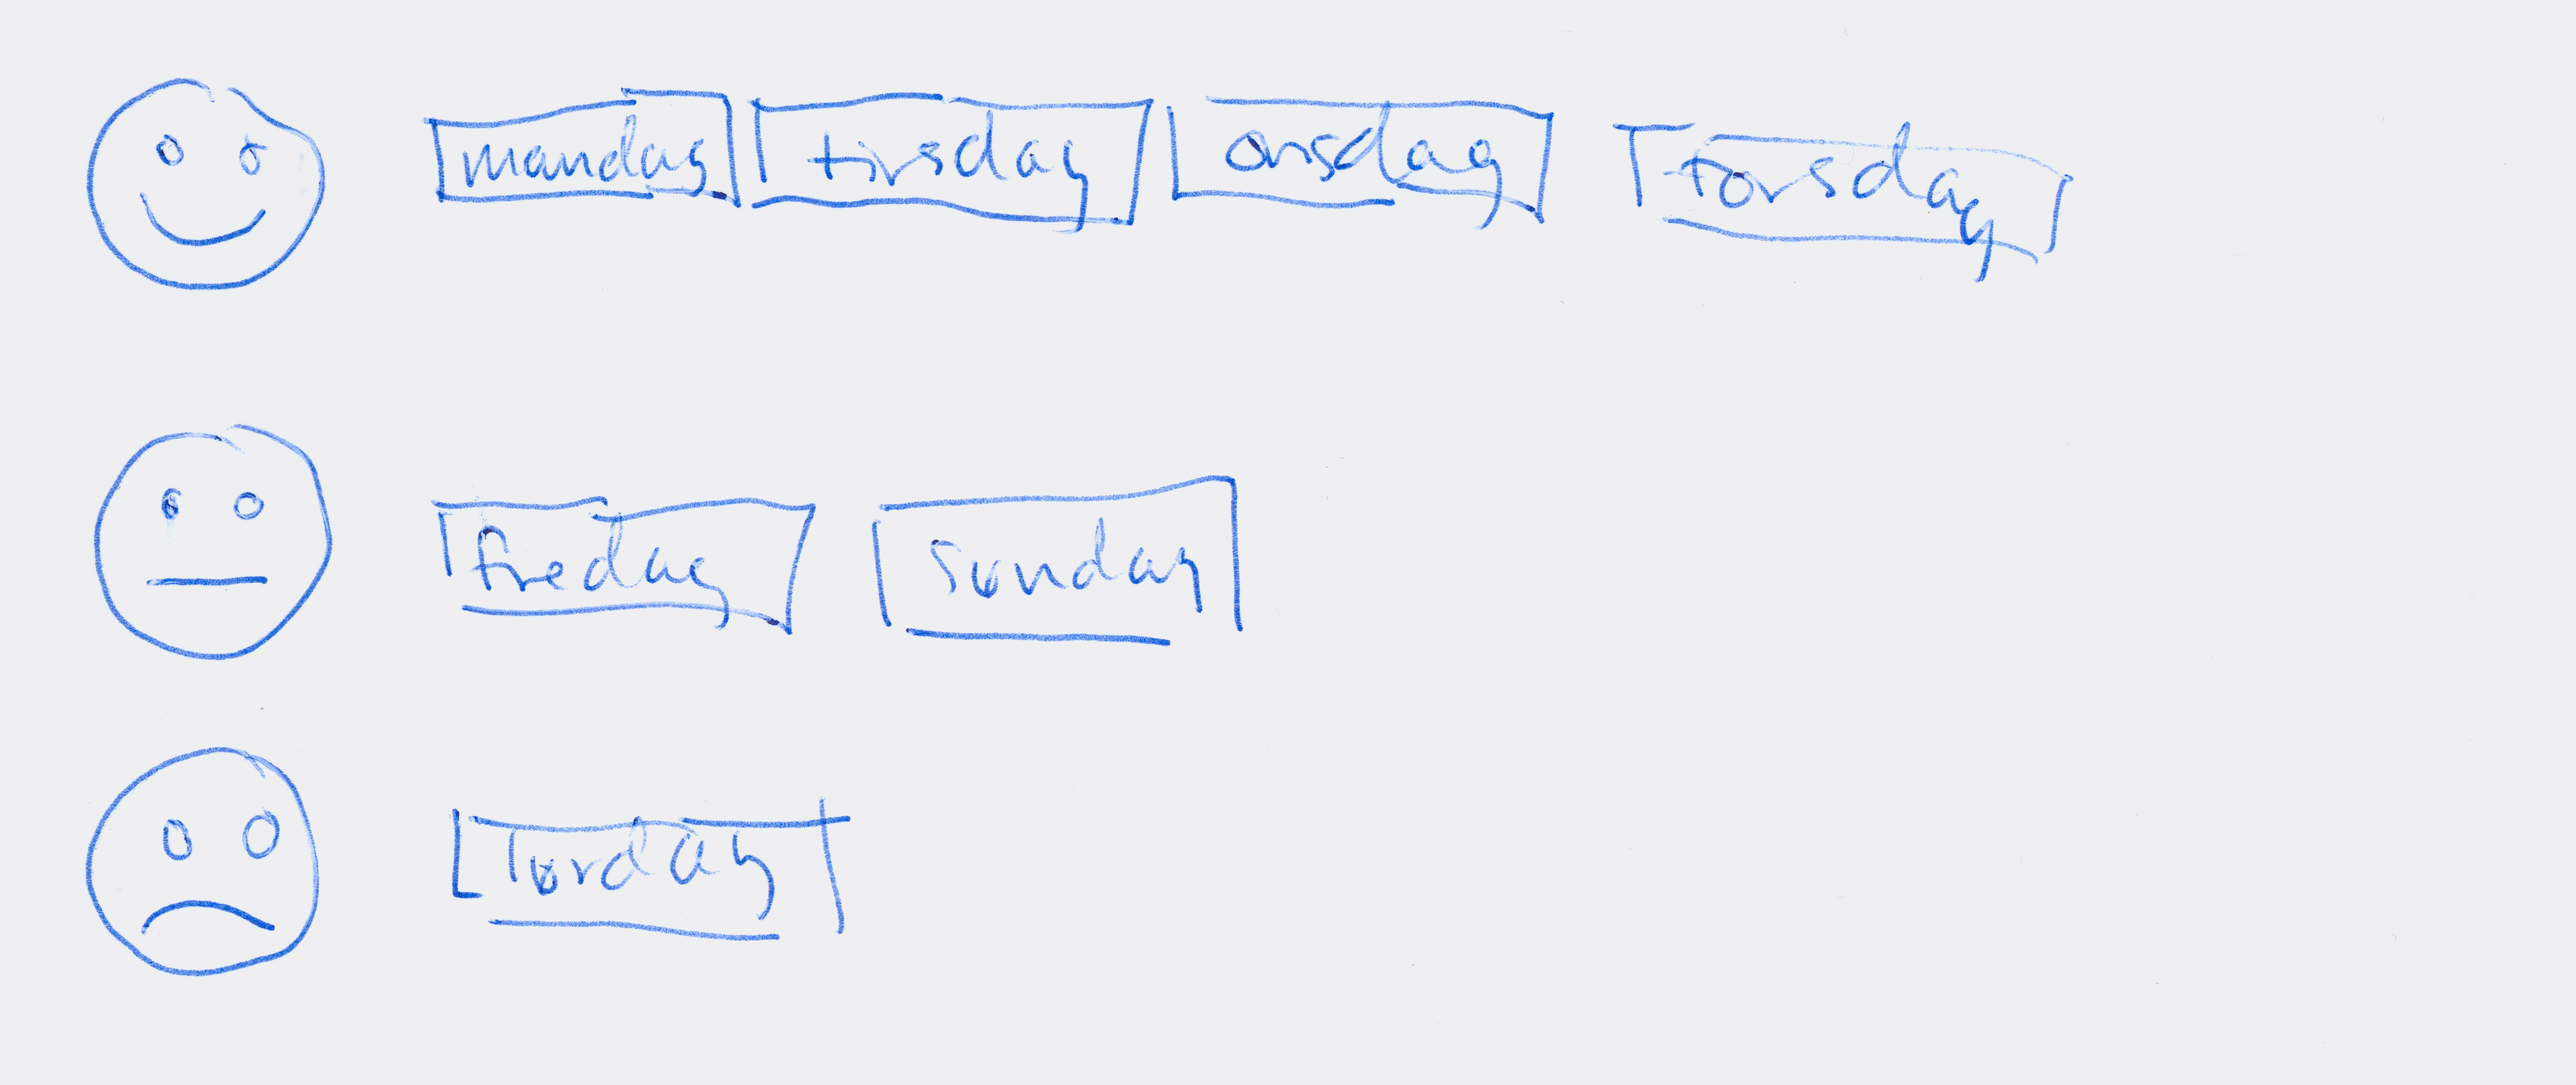
\includegraphics[width=0.7\textwidth]{smileyWeekSketch.png}
		\caption{\footnotesize Overview chart with each day classified into one of three categories.}
		\label{fig:smileyWeek}
\end{figure}

A more complex version of the above chart, see Figure~\ref{fig:detailedWeek} is to show a square for each hour, while still using the same classification into sad and happy smilies. Each day square contains 24 smaller squares that represent each hour of the day. The small hour squares are coloured with a gradient to show the activity level for that hour. With this chart the user can get an overview of the week as a whole, and identify what hours of the inactive days had the most sedentary behaviour. It also lets the user compare hours from multiple days as stated in requirement IR-4.

\begin{figure}[h!]
	\centering
		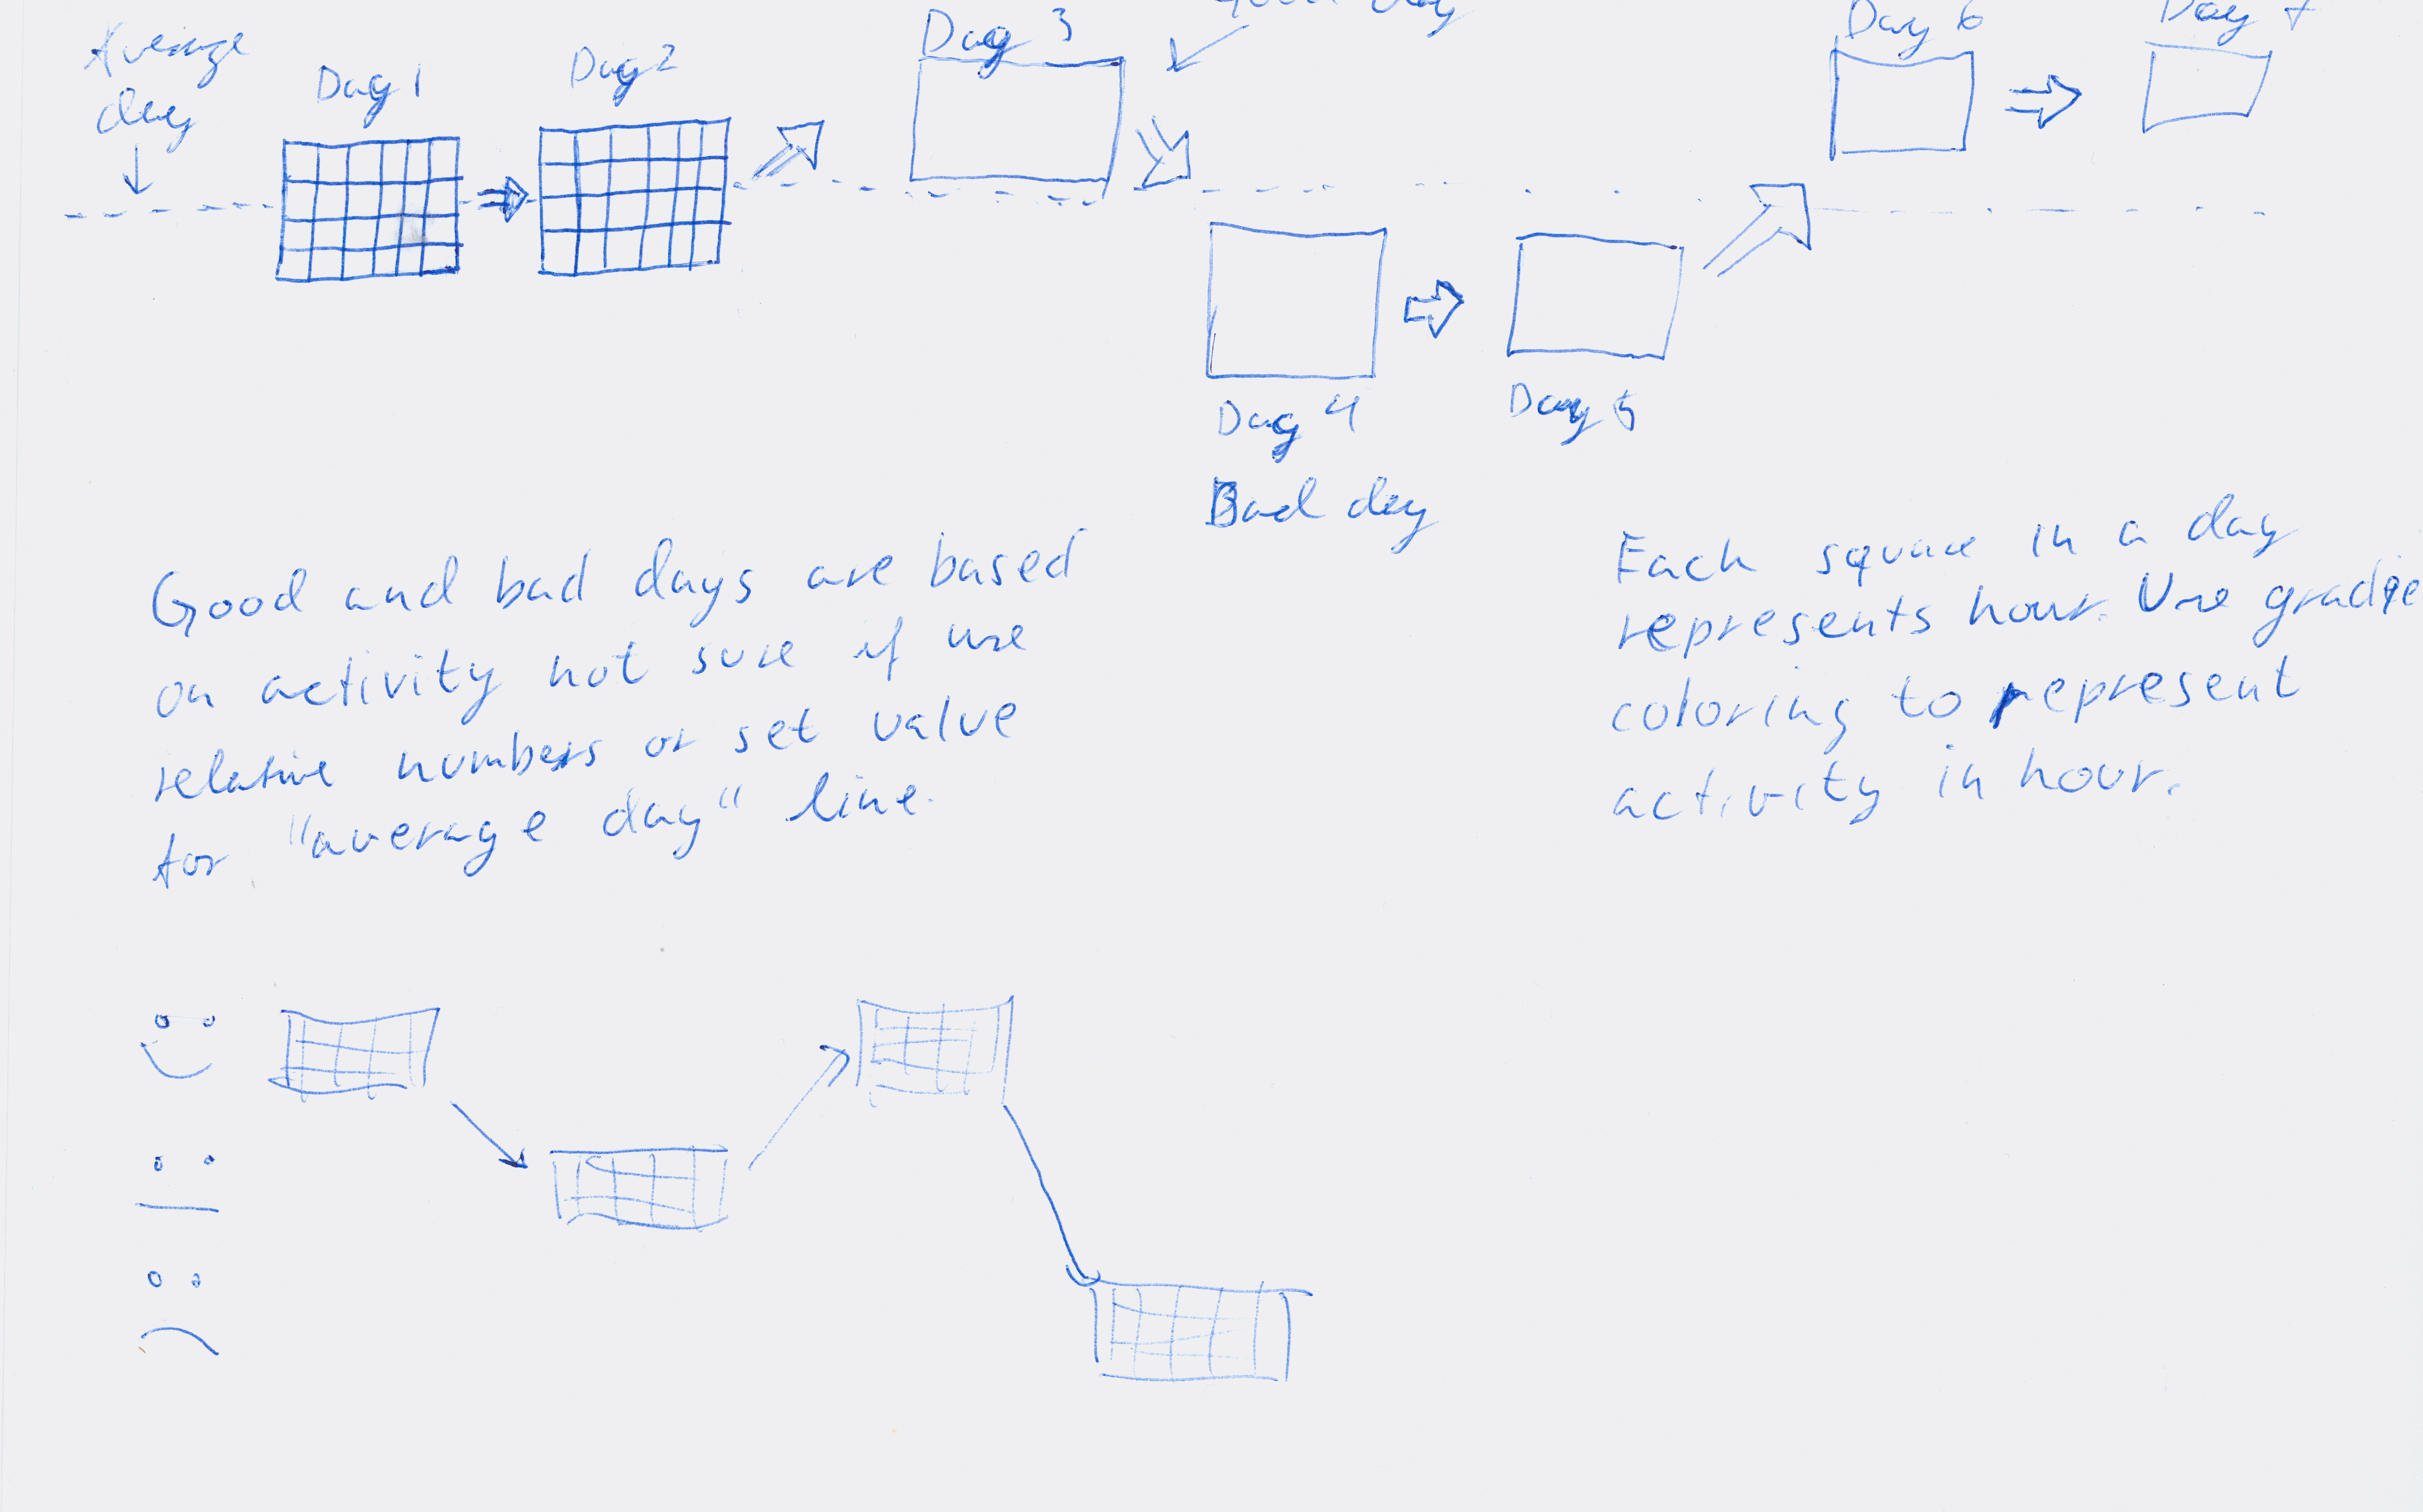
\includegraphics[width=0.6\textwidth]{detailedWeekSketch.png}
		\caption{\footnotesize A more detailed overview chart that classifies the days}
		\label{fig:detailedWeek}
\end{figure}

\subsection{Aggregated charts}
These type of charts show the sum of time spent sedentary, standing, and walking. Summing over the three classifications makes it easy to get an overview of the day as a whole. The drawback is that details are lost and it is not possible to pinpoint when each activity occurred during the day. Aggregated charts were created to cover the summary of daily activity requirement, IR-2. Aggregated charts can be used to get a general overview of the daily activity before spending time looking at more detailed visualizations. Additionally it can serve as an alert for patients with low activity levels, where the majority of the chart would be filled with inactivity.

Aggregated charts make use of two visual variables: Size and colour. The quantitative characteristic of size is used to determine the amount of each type of activity. For example for a pie chart, looking at the size of the pie slices we can quickly see how the different activity types compare to each other. The selective characteristics of colour is used to separate the different types of activity from each other. Since there are only three different type of activity, it is easy to distinguish between the different colours. 

\subsubsection{Pie chart}
The pie chart is a standard way of showing the amount of time spent in each activity state. Due to the familiarity of the pie chart it will be easy to understand for both users and patients. A legend shows which colour represents each type of activity. The exact percentage for each activity state is also displayed.

\subsubsection{Symbolic}
A more symbolic approach (see Figure~\ref{fig:symbolicPie}) is to remove the legend and instead use illustrations to convey which colour corresponds to which activity. To get more space for the illustrations the diagram uses boxes instead of pie slices to represent the distribution of each activity level. Though the box chart is not as much used as the pie chart, humans can intuitively compare sizes of different types of shapes as long as they are placed in close proximity. 

\begin{figure}[h!]
	\centering
		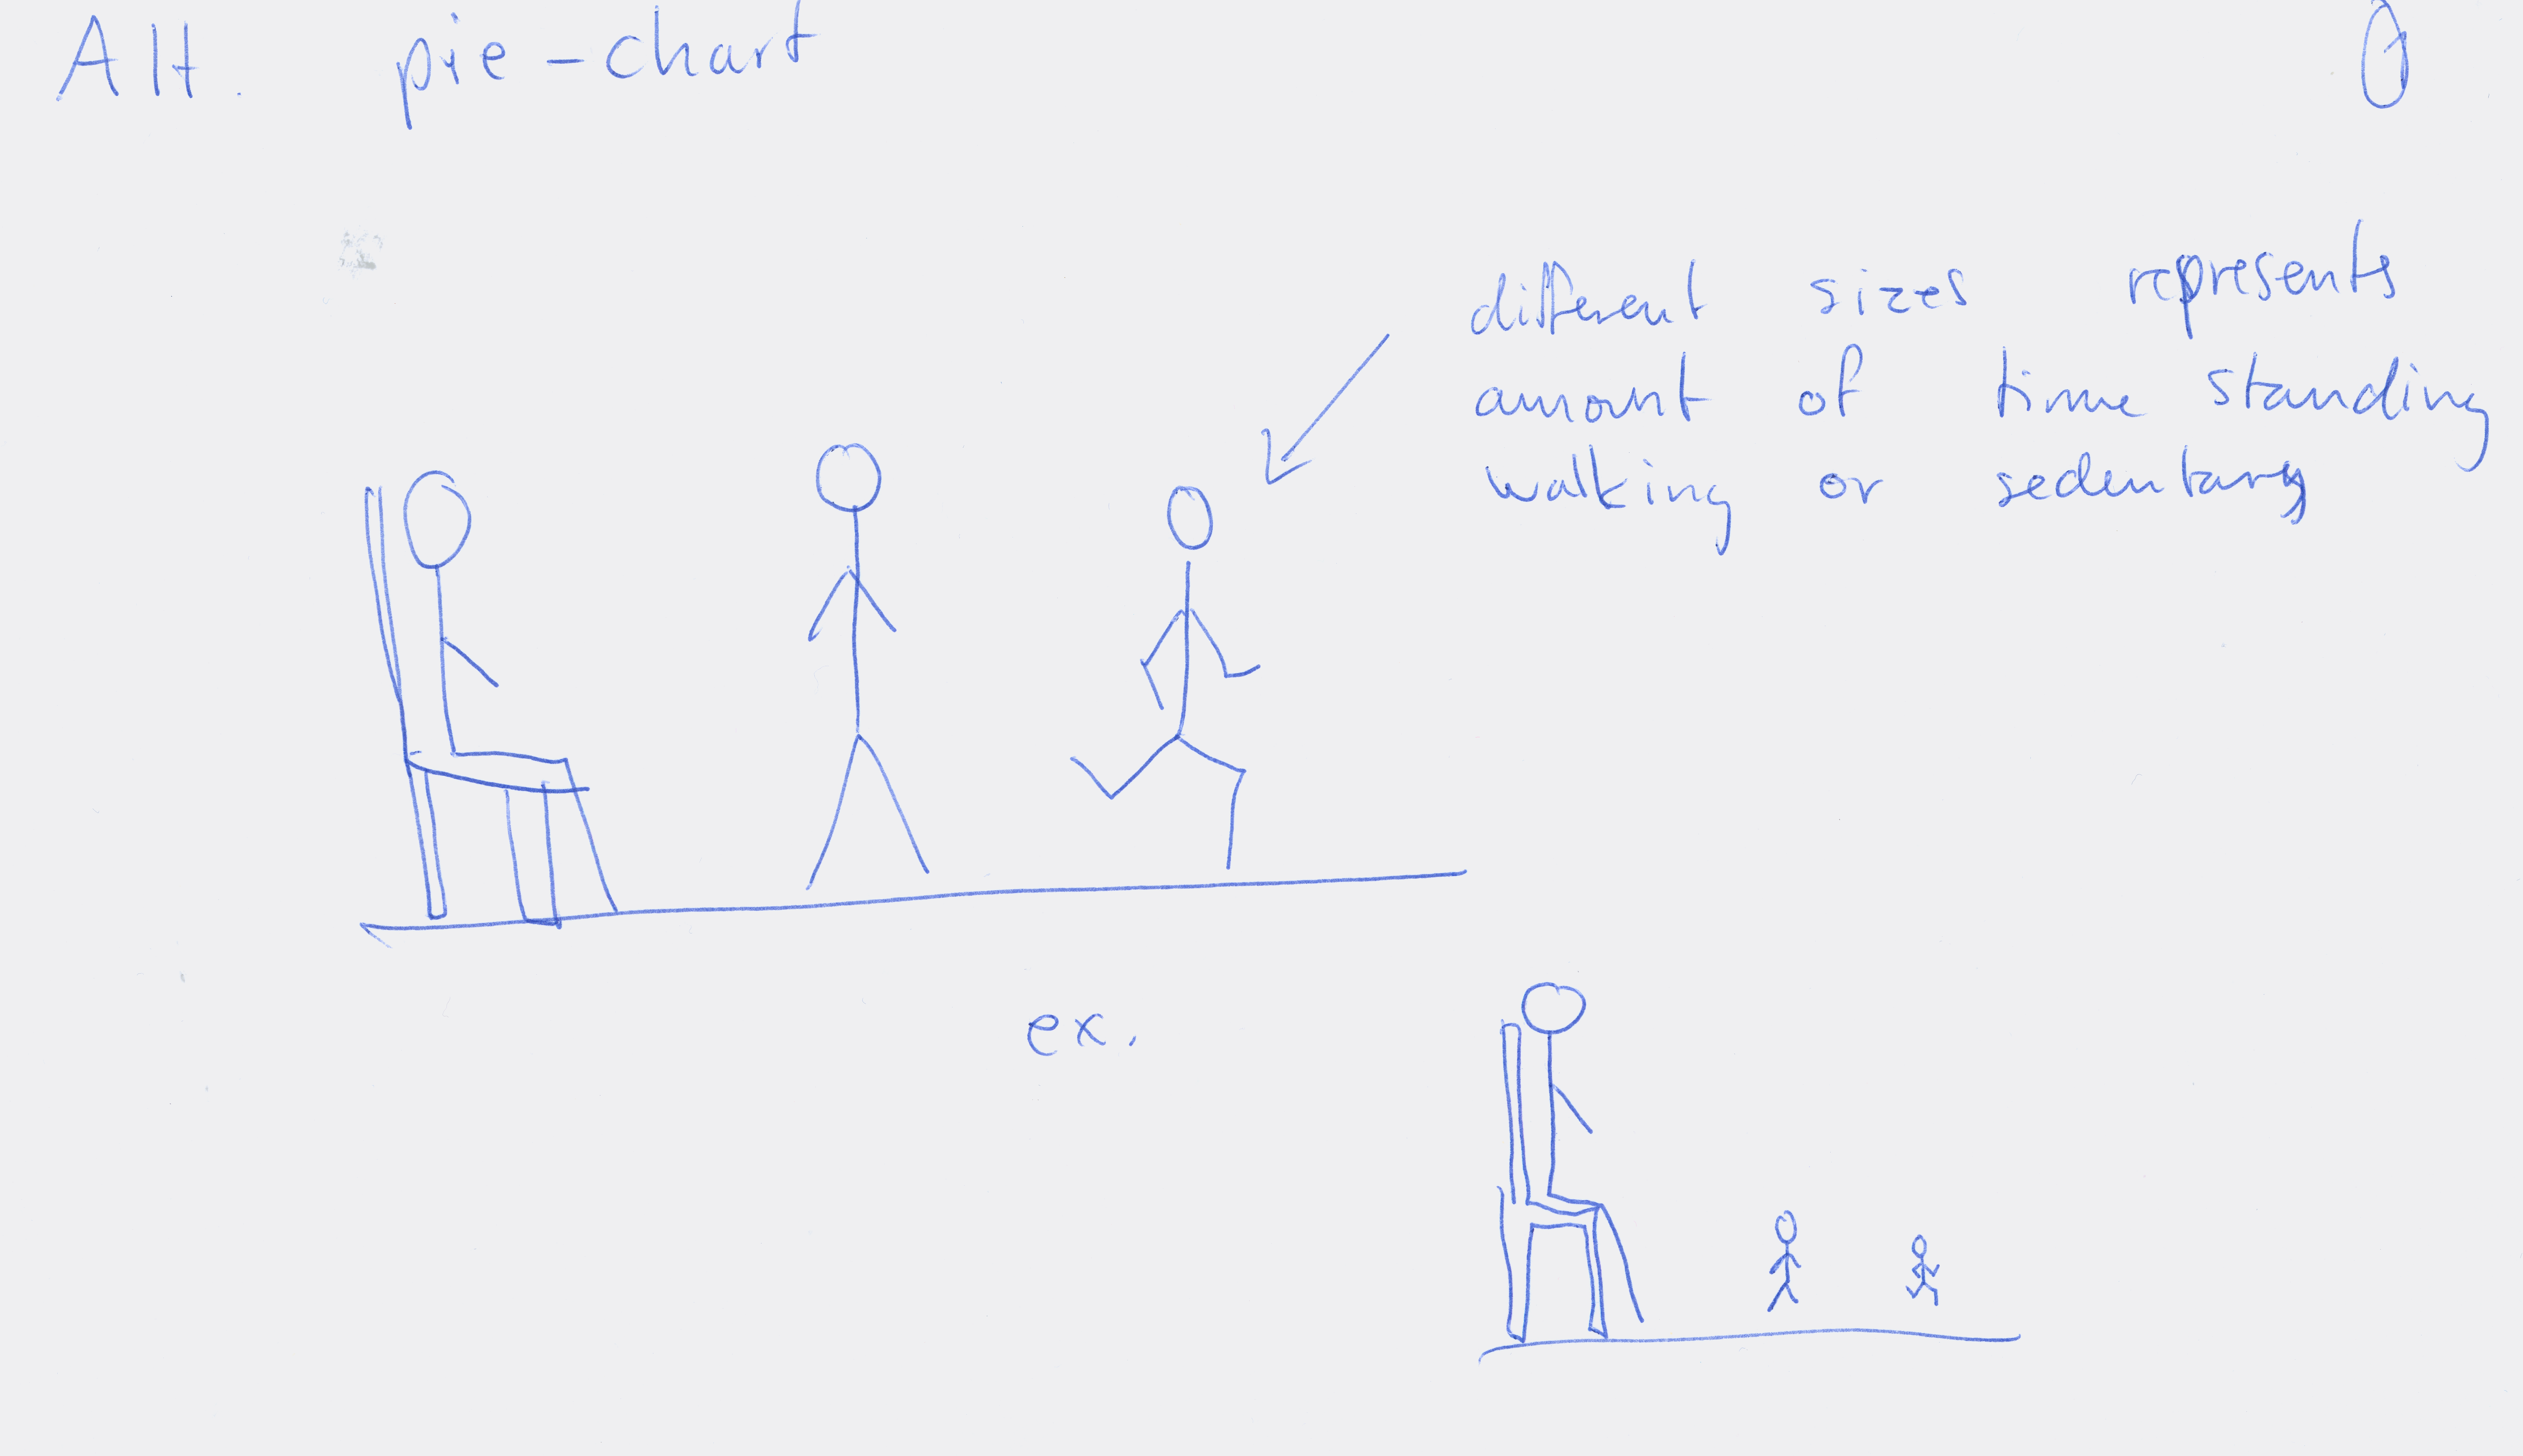
\includegraphics[width=0.7\textwidth]{stickSketch.png}
		\caption{\footnotesize Our first idea for a symbolic ``pie chart''.}
		\label{fig:symbolicPie}
\end{figure}

\subsubsection{Ball chart}
An alternative to the previous aggregated charts is to include more detail into a pie chart style, by using balls instead of normal pie slices. The balls are colour coded so that each colour reflects an activity state, while the sikze of the ball represent the continuous amount of time spent in the corresponding state. Each ball represents an interval of one of the classifications, so that many balls of one colour both represents the amount of that behaviour and shows how long each period of that behaviour was. This can also be used to identify if a user is active during the night, which is requirement IR-7. Figure~\ref{fig:ballChart} shows an example of such a graph. The benefit with this type of graph is that one can easily identify long periods of sedentary behaviour. Taking small breaks with movement can help ``split up'' those balls, which is beneficial for ones health. By adding interactivity to the chart the user can select each ball and see what time it corresponds to. Overall the chart allows for the large balls to be easily spotted and efficiently discovery when the incident occurred.

\begin{figure}[h!]
	\centering
		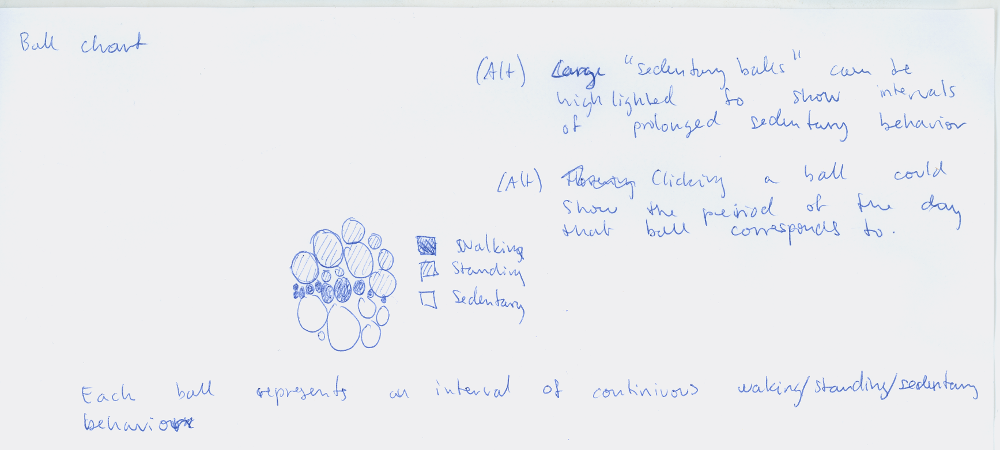
\includegraphics[width=0.7\textwidth]{ballChart.png}
		\caption{\footnotesize Rough drafts of the Ball chart.}
		\label{fig:ballChart}
\end{figure}

\subsection{Timeline charts}
Timeline visualisations are effective at illustrating when various activities occurred during the day. Timelines use a long horizontal bar that has different colours for different behavioural classification. These visualizations primarily address requirements IR-3, IR-4, IR-5 and IR-6, which state the need to show and compare minutes and hours during the day. Timeline charts can also be used to identify patients that are active during the night, which is requirement IR-7.

The timelines we sketched all make use of the visual variable position. The position either on a rectangle or on a circle, represents what time of the day activity occurred. Continuous timelines, as seen in Figure~\ref{fig:clocks12}, make use of the selective characteristic of colours to show what type of activity occurred at any point of the day. The blocked timeline, as seen in Figure~\ref{fig:timelineBlocks}, makes use of the visual variable value to convey the amount of activity for each respective hour of the day. Since value can be ordered, it is easy to see which hours have activity, and that one hour has more activity than another. Value is not qualitative however, so finding one hour with twice as much activity as another is difficult.

\subsubsection{Continuous}
One approach to this visualization type is to create a continuous timeline that contains every little detail of activity. The continuous timeline is useful for quickly identifying periods of the day with unsatisfactory behaviour, but the detail can also be distracting and make it hard to read the diagram.

\subsubsection{Blocks}
Instead of having a continuous scale, a blocked approach can be used, as seen in Figure \ref{fig:timelineBlocks}. The timeline would be divided into 24 blocks, each block corresponding to an hour of the day. A gradient colour scale is used to represent the amount of activity inside the hour block. This makes it easy to identify hours of the day where the patient is sedentary. 

\begin{figure}[h!]
	\centering
		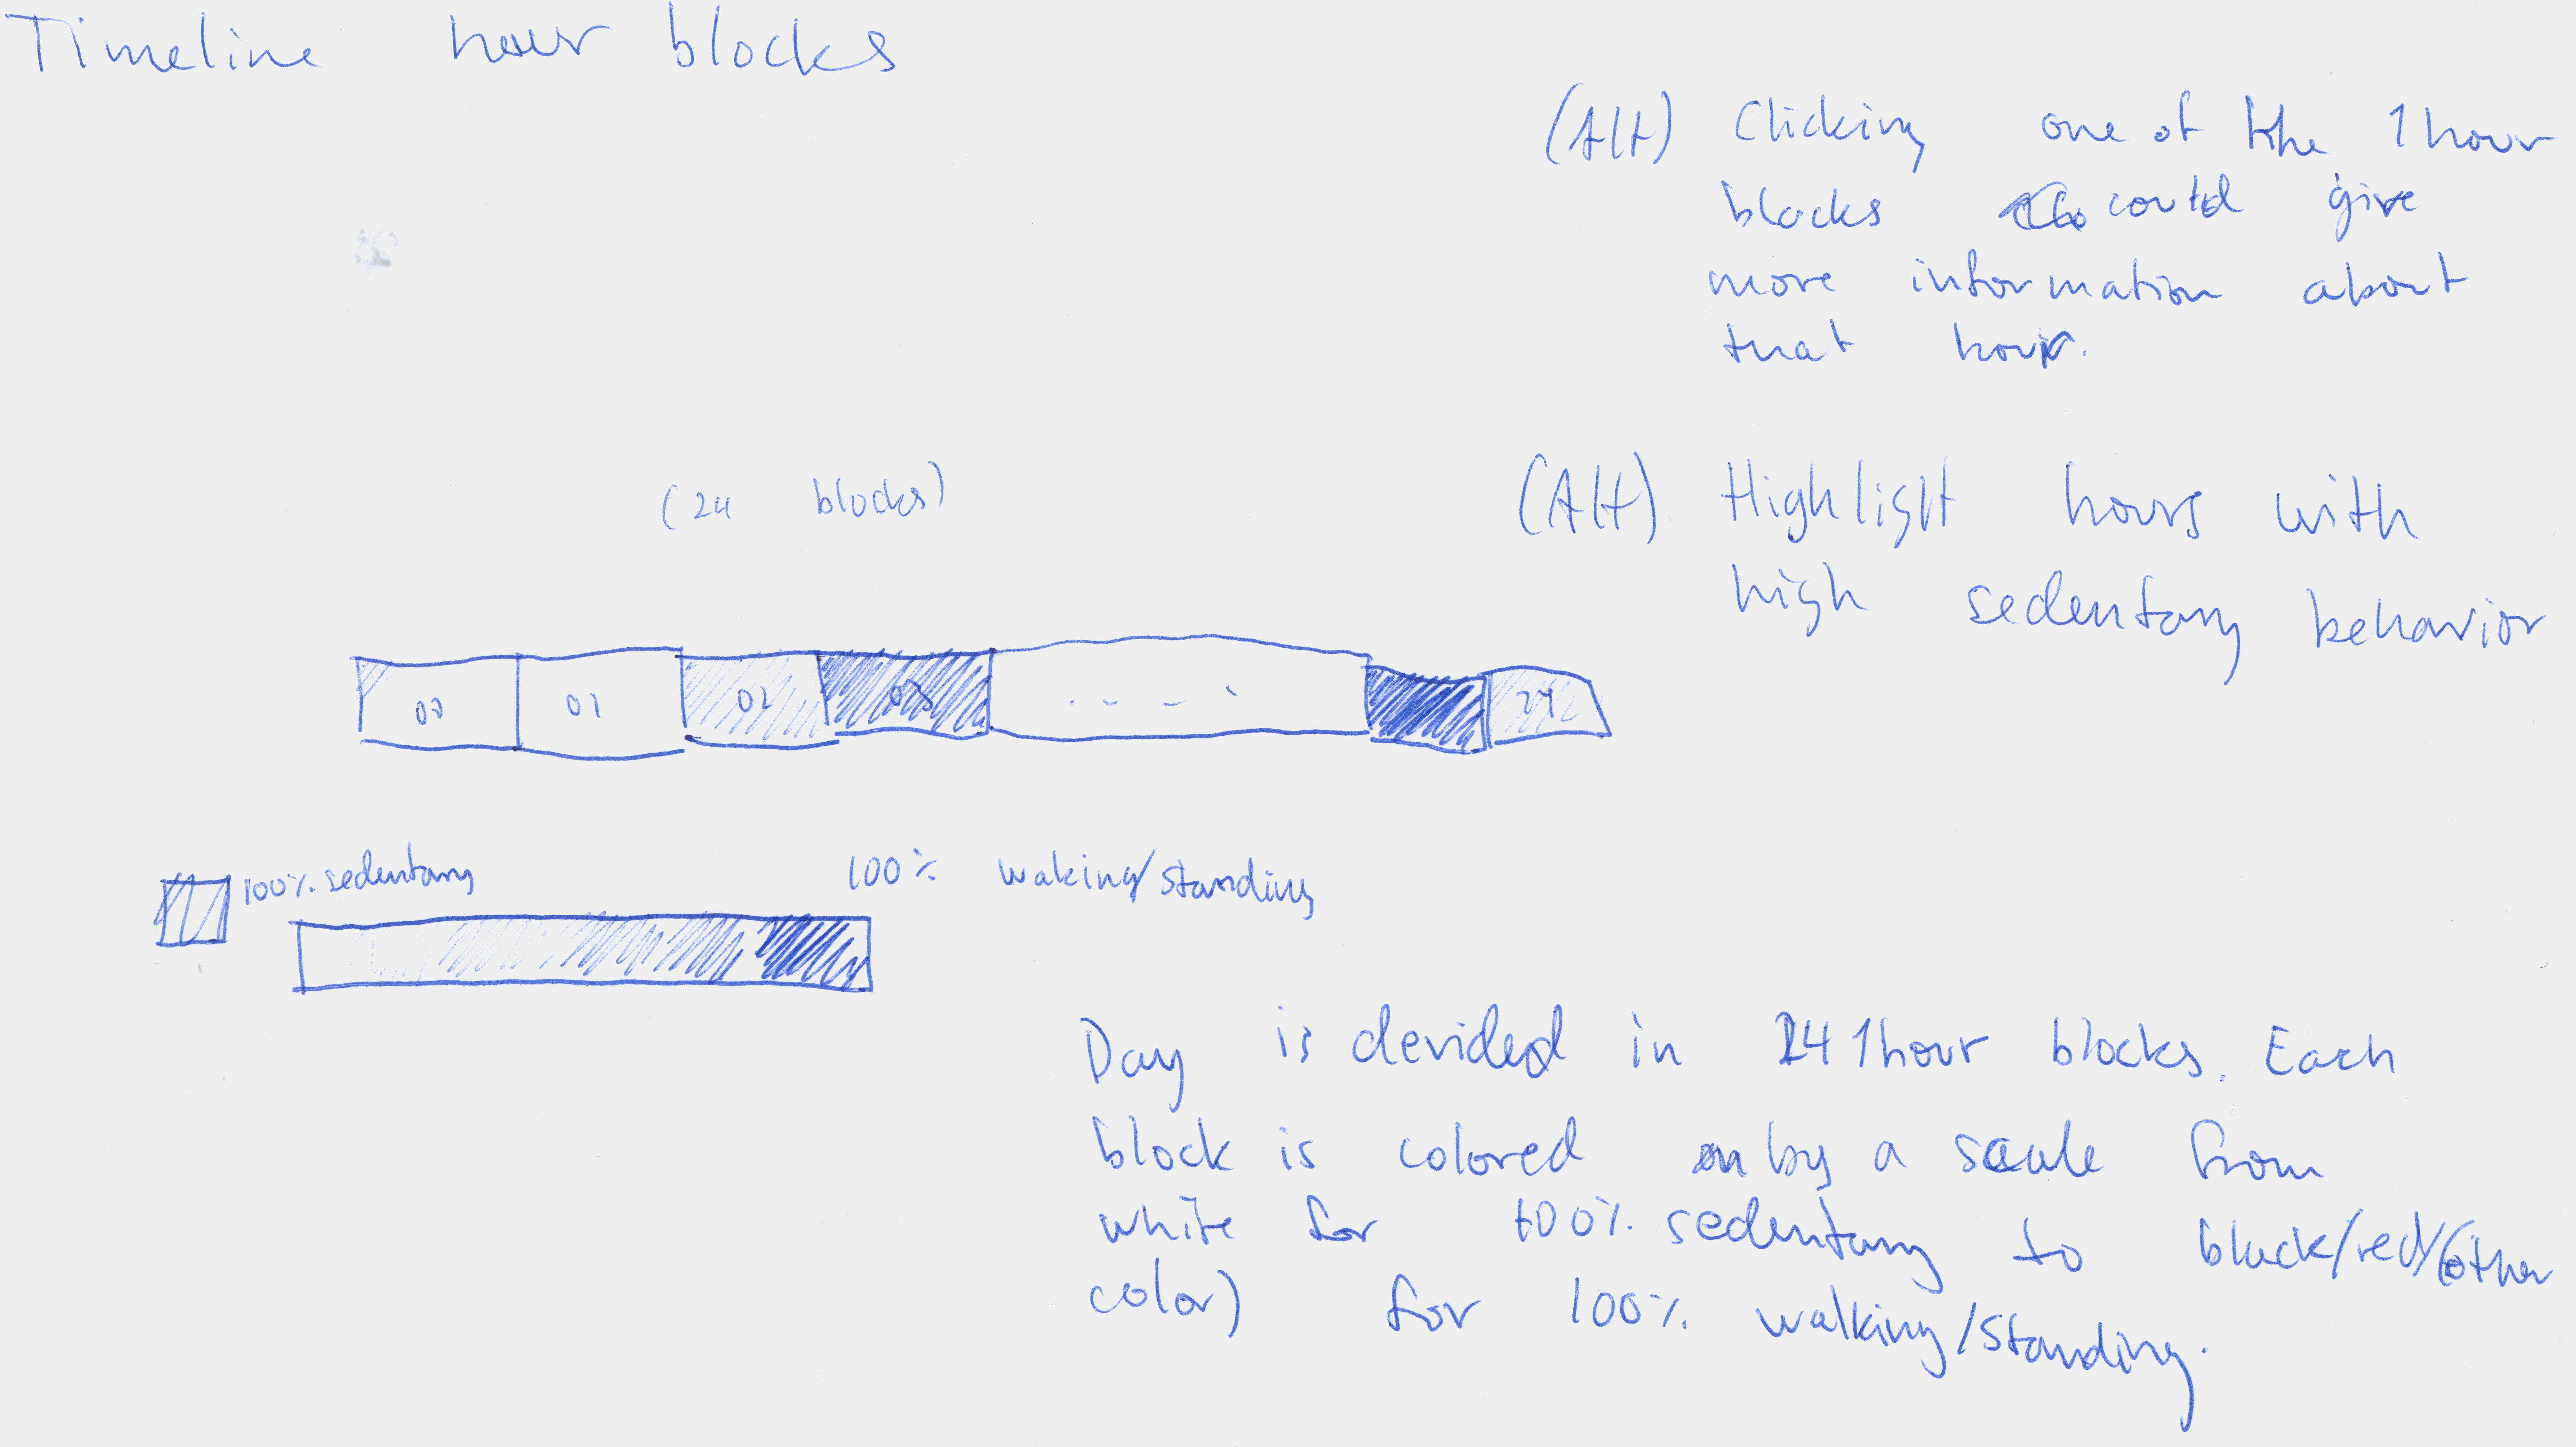
\includegraphics[width=0.7\textwidth]{timelineBlocksSketch.png}
		\caption{\footnotesize Timeline with hour blocks}
		\label{fig:timelineBlocks}
\end{figure}

\subsubsection{Clock}
A timeline may need some explanation before the user understands it properly. By creating two clocks instead of a long horizontal bar the user can more intuitively understand what the visualization is presenting. Since a clock has only 12 hours, two clocks are created to represent the entire day. To make it easier to identify day and night, a descriptive background is necessary, see Figure \ref{fig:clock12}.

\begin{figure}[h!]
	\centering
		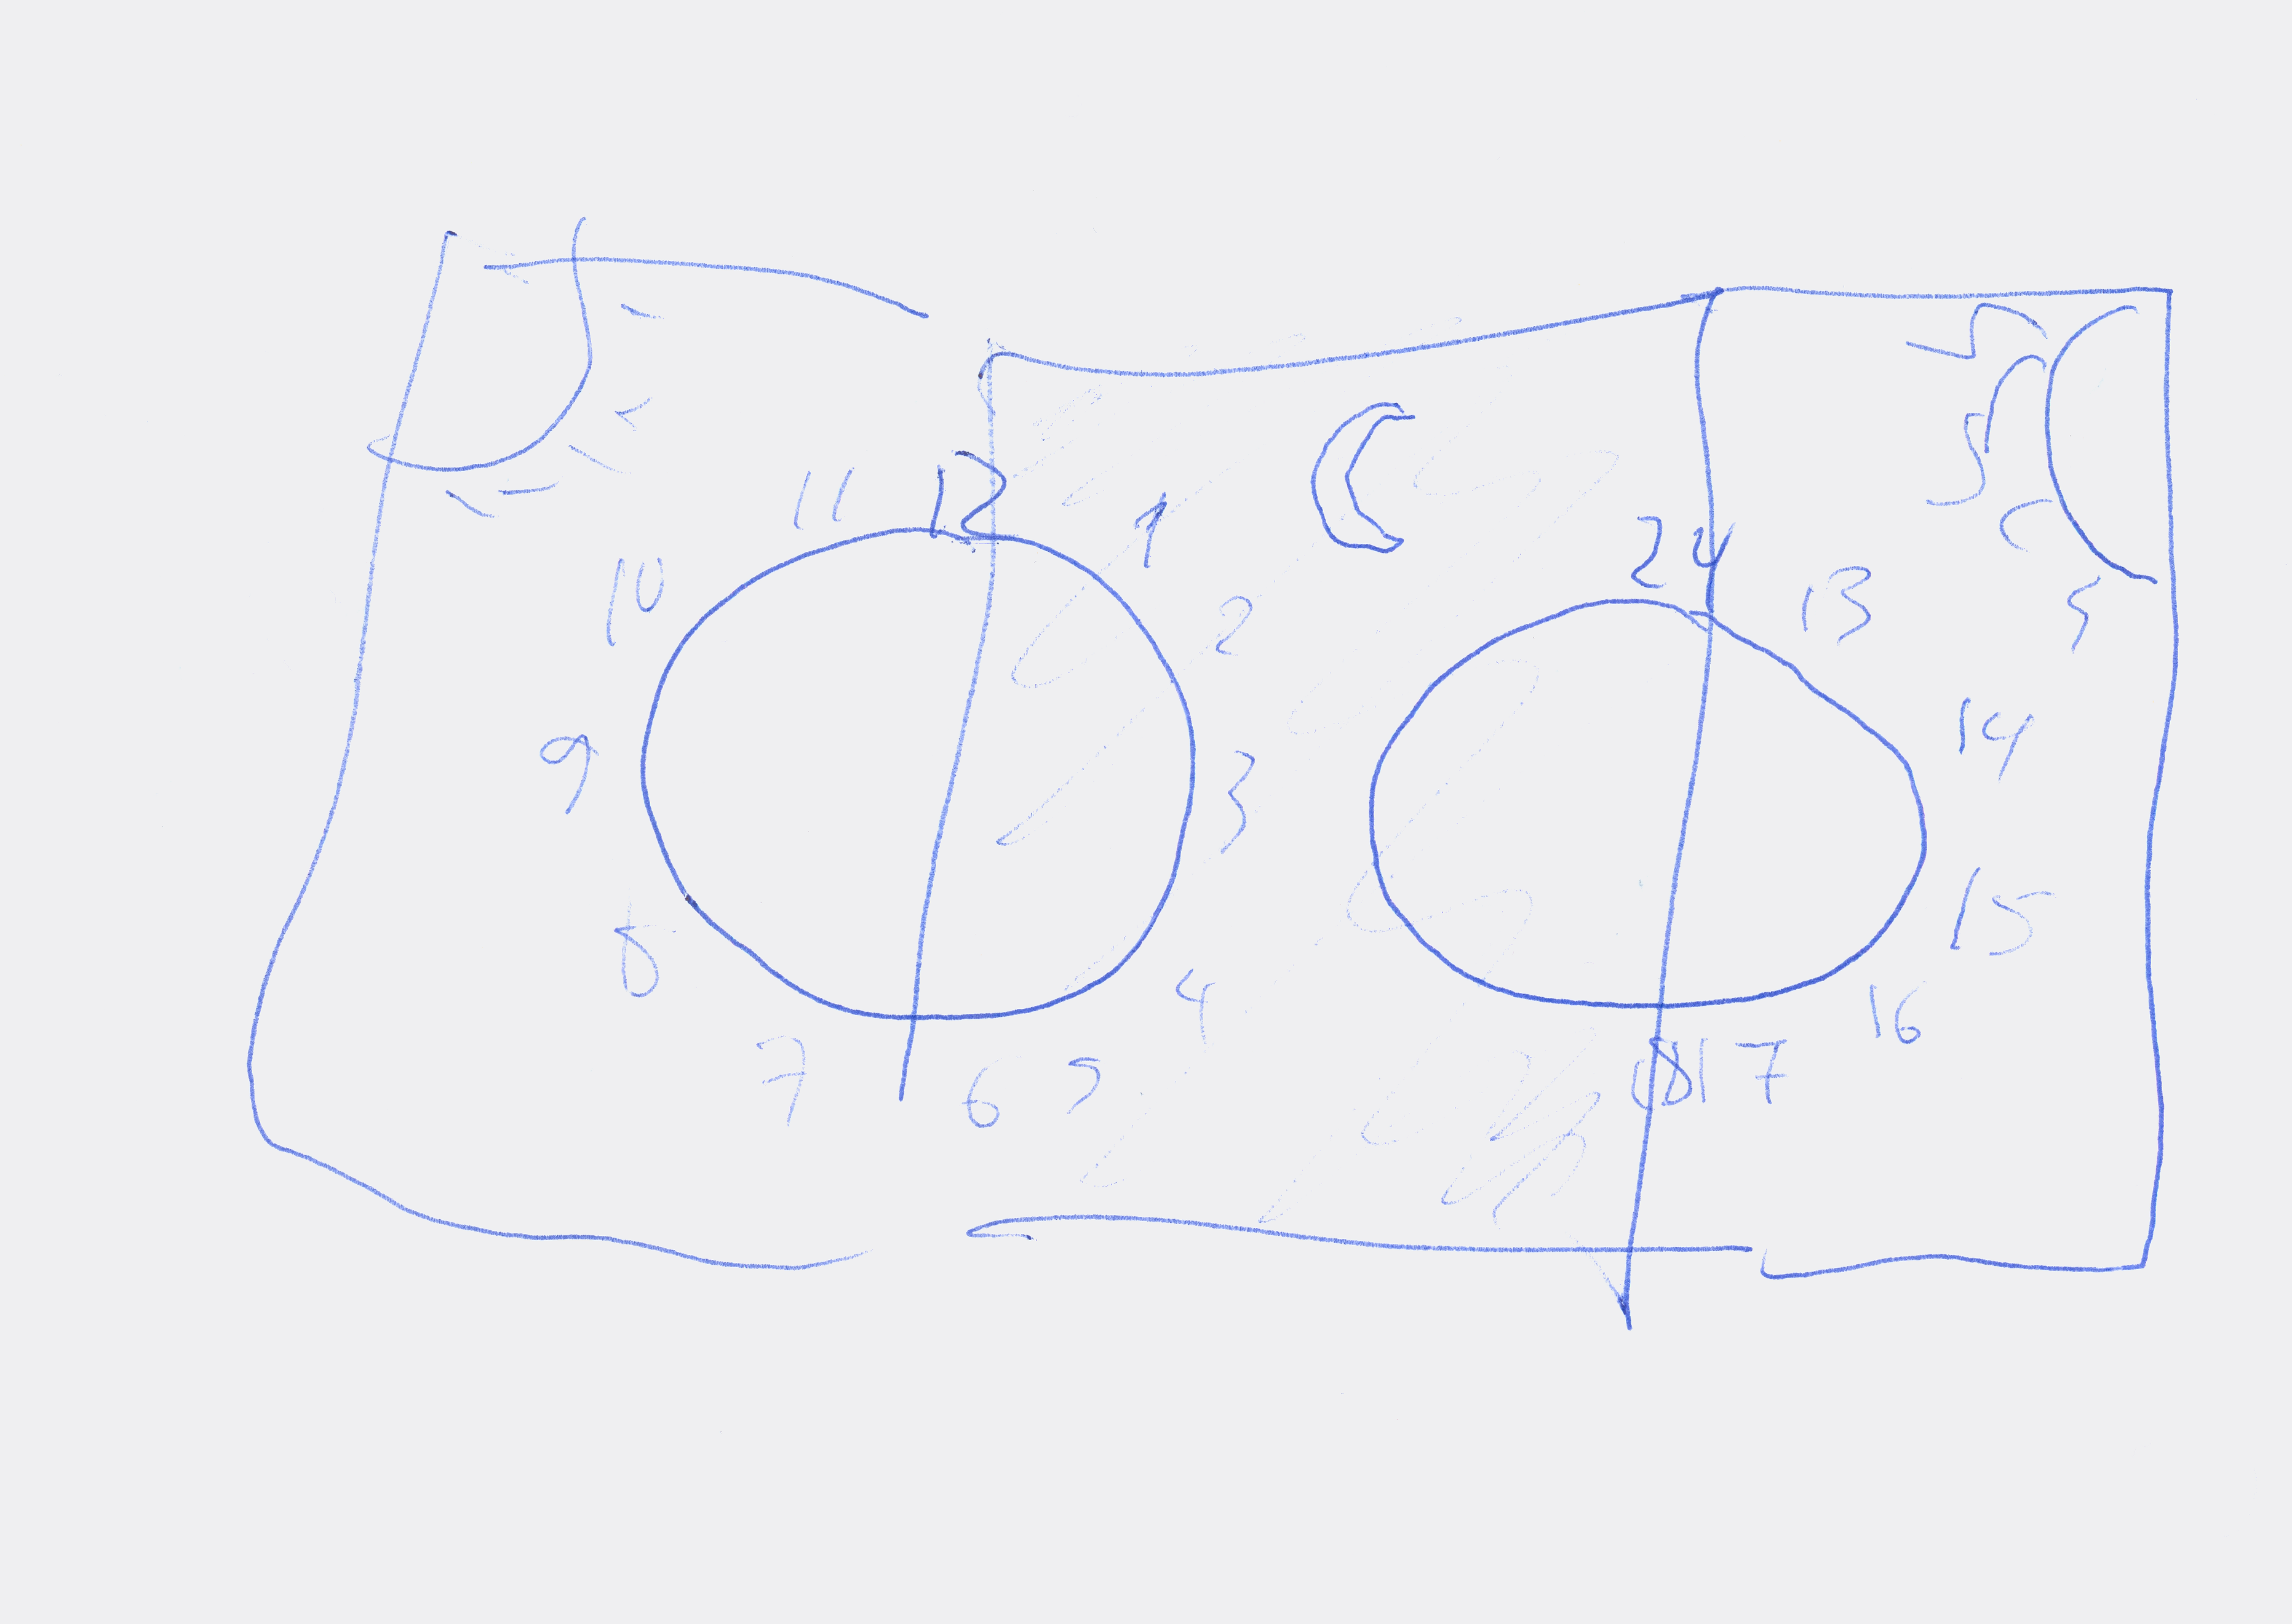
\includegraphics[width=0.7\textwidth]{clock12Sketch.png}
		\caption{\footnotesize Two 12 hour clocks show the activity of the day.}
		\label{fig:clock12}
\end{figure}

Another approach is to use one 24 hour clock. This makes it easier to see the transition between AM and PM, but 24 hour clocks are not natural, so it might be problematic for the user to understand.

\section{Programming framework}
The task was to create custom visualizations from data gathered by the activPAL sensor. The choice of programming tools fell on HTML5 and an open source JavaScript framework called D3js.

\subsection{HTML5}
HTML is a markup language for the creation of web pages. HTML describes the structure and the contents of the web page. In later years, the need for advanced styling and complex interaction with web pages has made CSS and JavaScript increasingly popular. HTML5 was created as a response to this, HTML5 is an umbrella term for creating web pages using HTML5, CSS3 and JavaScript.

HTML5 has simplified the syntax compared to earlier versions. New tags have been added to better represent the modern web page elements. Other features include media tags which greatly simplifies adding multimedia content, such as playing audio and video files. More importantly for our project is the extensive support for interactive and animated graphics through the \emph{canvas-} and \emph{svg}-tag.

The new features of HTML5 and CSS3 make it much easier to create web applications for multiple platforms and screen sizes. After the smartphone and tablet revolution, creating responsive and adaptable websites has become more important. Additional new features in HTML5 give a large amount of flexibility with respect to the user interface and graphical visualizations.

\emph{Cascading Style Sheets} (CSS) is a language used to describe the styling of an HTML document. CSS documents describes the size, color and look of HTML elements. A new feature in CSS3, which is part of HTML5, is \emph{Media Queries}. With Media Queries it is possible to specify different styling relative to the size of the screen. This functionality is useful when creating applications that target devices with different screen sizes, such as smartphones, tablets and laptops. 

\subsection{Data-Driven Documents}
JavaScript is the main scripting language for web pages. It is a client-side scripting language that allows programmers to add functionality to otherwise static HTML-pages. While CSS3 takes care of the styling of HTML-elements, JavaScript is used to create customized behaviour. All modern browsers have JavaScript engines/interpreters that compile and run JavaScript code.

JavaScript is now an industry standard maintained by ECMA International. The standardized version of the script is named ECMAScript. Today, the names ECMAScript and JavaScript are used interchangeably, and JavaScript is often used to refer to ECMAScript. Because different browsers have different implementations of the JavaScript engine, slight variations in the way JavaScript code will run on these browsers exists.

Together with HTML5 and CSS3, JavaScript is great for creating web applications that can be designed to run on both mobile and stationary devices. JavaScript has a multitude of useful open source libraries that can be used to create complex user interaction, animation, and custom graphics.

One of the challenges in this project was to create different visualizations to represent the activity patterns of patients. Creating custom graphics in HTML5 can be done using both the canvas- and the svg-tag. In this project \gls{svg} is used. \gls{svg} is an image format that uses XML encoding to define shapes, lines, colors, and text. One benefit of svg, compared to other image formats, is that details in \gls{svg}-images will not be lost when zooming. All popular browsers, and most mobile devices, support rendering of \gls{svg}-images.

Creating graphics using svg-tags directly is cumbersome and time consuming. \gls{d3} is an open source framework that greatly simplifies this task. \gls{d3} is written in JavaScript and designed to be used in combination with HTML5. The framework can be used both to create new \gls{svg} images from scratch or modify and edit existing images. Another feature is the ability to easily add interactivity and animation to the \gls{svg}-elements. HTML5 in combination with \gls{d3} gives us flexibility to create almost any type of visualization and adding interactivity and animation to it.

% REVIEW
\section{Running prototype}
\label{sec:runningPrototype1}
Nine of the paper sketches were selected for implementation, so they could be presented to the first focus group. Some changes were made and additional functionality was added to the implemented versions of the visualizations, such as highlighting and different view modes. All diagrams were given IDs as seen in Table~\ref{tab:runProtDesc1}.

\begin{table}[h!]
  \begin{center}
  \begin{tabular}{|c|c|p{10cm}|}
    \hline
    \textbf{ID} & \textbf{IR} & \textbf{Description}\\ \hline
    U1 & 1 & Classifies each day of the week into one of three categories: High, medium and low activity. \\ \hline
    U2 & 1, 3, 4, 7 & Classifies each day of the week as in U1. Also shows 24 squares for each day, each square representing an hour. The activity level for each hour is displayed using a gradient. \\ \hline
    F1 & 2 & Pie chart showing the amount of activity for each day. \\ \hline
    F2 & 2 & Same as F1, but with boxes instead of pie slices and descriptive figures inside each box.  \\ \hline
    F3 & 2, 7 & Ball chart. Divides the pie slices of F1 into bubbles, each bubble representing one interval of activity. \\ \hline
    T1 & 3, 4, 7 & Timeline of 24 squares, each square represents one hour of activity. The amount of activity in that hour is displayed using a gradient. \\ \hline
    T2 & 5, 6, 7 & Rectangle shaped timeline, showing the activity type using colour coding.  \\ \hline
    T3 & 5, 6, 7 & Two 12-hour clocks showing the activity type using colour coding. \\ \hline
    T4 & 5, 6, 7 & One 24-hour clock showing the activity type using colour coding. \\ \hline
  \end{tabular}
  \end{center}
  \caption{Diagrams implemented in the first prototype.}
  \label{tab:runProtDesc1}
\end{table}

The two diagrams U1 and U2 (see Figure~\ref{fig:uFirst}) are overview charts. These are designed to give a quick overview of the week. U2 experiments with adding more detail, and contains 24 small squares for each day that represent the activity of each hour. Holding the mouse cursor over a day in U1 will show the percentage of each type of activity for that day. Holding the mouse cursor over a square in U2 will show the percentage of each type of activity for the hour that the square represents. These diagrams satisfy requirement IR-1, which states that the visualizations should give an overview of the week. U2 also shows the hourly activity level for each day, meaning patients that are active during the night can be identified, and lets the user compare hours from multiple days as stated in requirement IR-7, IR-3, and IR-4. 

\begin{figure}[h!]
  \centering
  \begin{subfigure}[b]{0.45\textwidth}
    \centering
    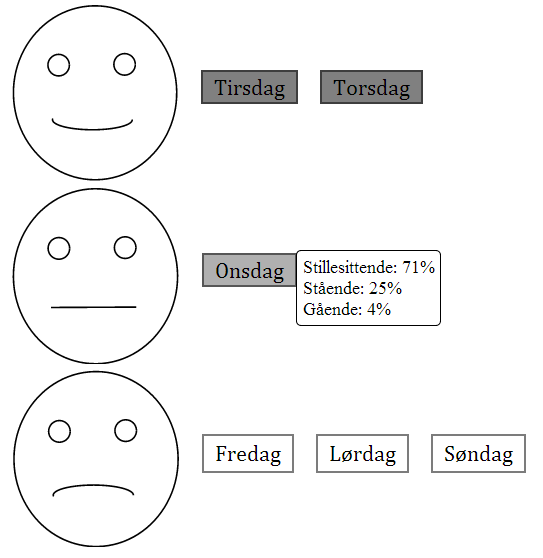
\includegraphics[width=\textwidth]{u1First.png}
    \caption{U1}
  \end{subfigure}
  \begin{subfigure}[b]{0.45\textwidth}
    \centering
    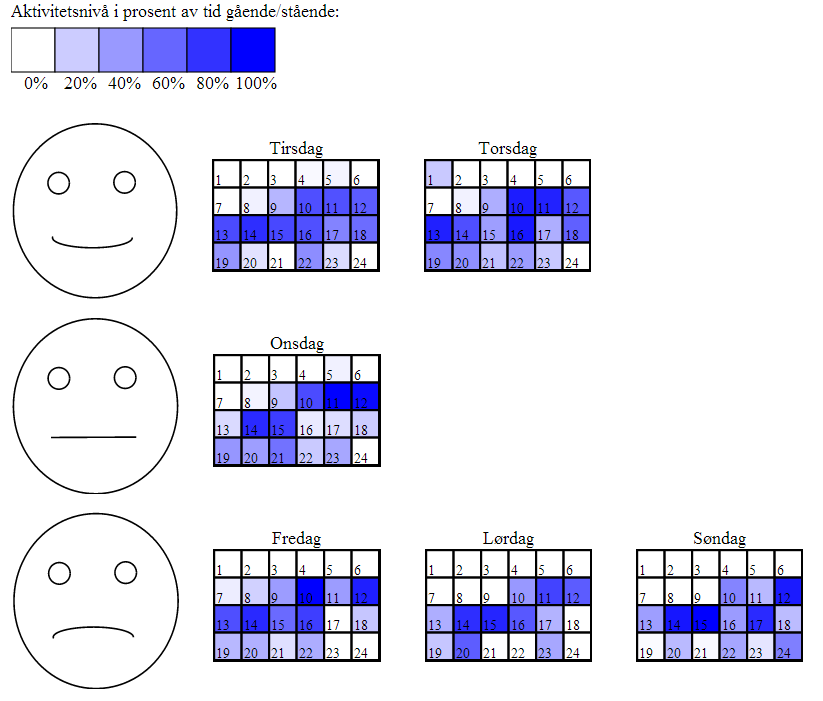
\includegraphics[width=\textwidth]{u2First.png}
    \caption{U2}
  \end{subfigure}
  \caption{\footnotesize Overview charts.}
  \label{fig:uFirst}
\end{figure}

Diagrams F1, F2 and F3 (see Figure~\ref{fig:fFirst}) are the aggregated charts. These diagrams shows the fraction of each type of activity for a day, requirement IR-2. F1 and F2 are similar, F1 is a standard pie diagram while F2 uses boxes with figures describing the activity. F1 and F2 has two types of view modes: one day or the entire week. F3 is more complex, this diagram shows each interval of activity as a ball. Long intervals of activity are represented by a larger ball than small intervals of activity. This graph can therefore be used both to see the distribution of the different activity types and, more importantly, the length of continuous activity, or sedentary behaviour. This is useful for identifying if the patient has very long periods of sedentary behaviour, or if the patient walks continuously for a long time. Holding the mouse cursor over a ball shows the time on which the activity interval occurred as well as the length of the interval. This enables the user to see if patients are active during the night as stated in requirement IR-7. F3 also offers a highlighting mode, where sedentary intervals longer than one hour are highlighted. 

\begin{figure}[h!]
  \centering
  \begin{subfigure}[b]{0.45\textwidth}
    \centering
    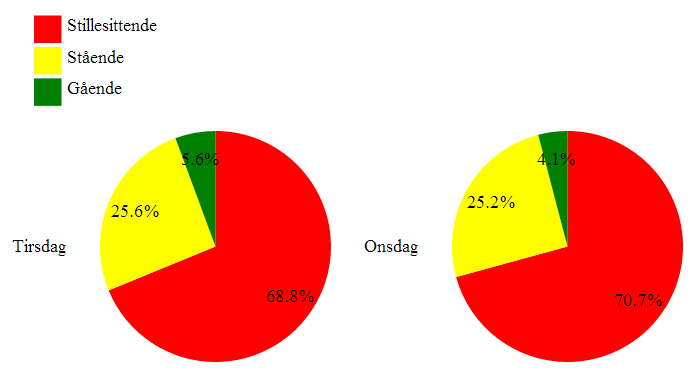
\includegraphics[width=\textwidth]{f1First.png}
    \caption{F1}
  \end{subfigure}
  \begin{subfigure}[b]{0.45\textwidth}
    \centering
    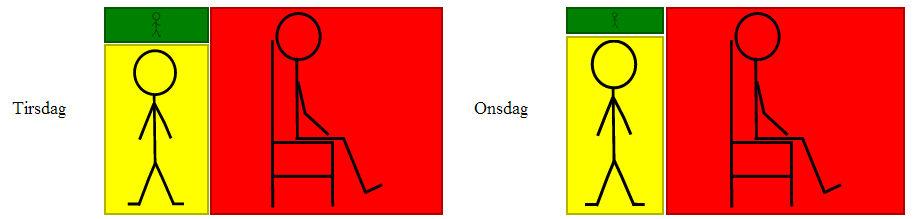
\includegraphics[width=\textwidth]{f2First.png}
    \caption{F2}
  \end{subfigure}
  \\
  \begin{subfigure}[b]{0.45\textwidth}
    \centering
    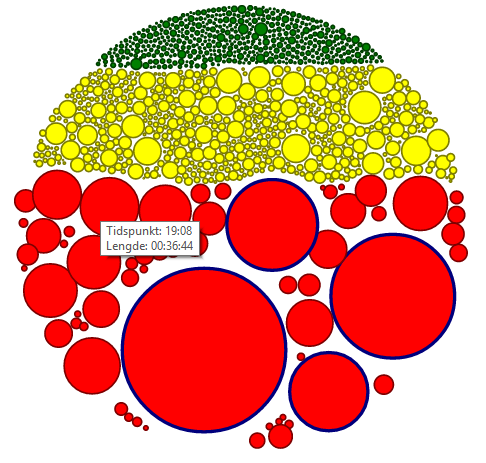
\includegraphics[width=\textwidth]{f3First.png}
    \caption{F3}
  \end{subfigure}
  \caption{Aggregated charts}
  \label{fig:fFirst}
\end{figure}

T1, T2, T3 and T4 (see Figure~\ref{fig:tFirst}) are diagrams that show timelines or clocks. These diagrams are useful to see when the patient was active during the day. T1 shows 24 squares each representing an hour of the day, as stated in requirement IR-3. The percentage of activity (walking and standing) is shown as a gradient in each square. Holding the cursor over a square displays the percentage of each type of activity. T2 is also a timeline, but here the data is not aggregated so the timeline is continuous and shows the activity at a much more detailed level, as stated in requirement IR-5. This is useful if the user needs to see when in a particular hour the activity was performed. It also distinguishes between standing and walking activity. T3 and T4 also show the activity continuously but they use a clock instead of a rectangle to illustrate when on they day the activity occurred. T3 uses two 12-hour clocks, while T4 uses a single 24-hour clock. Diagrams T2, T3 and T4 can toggle highlighting. When highlighting is toggled sedentary behaviour longer than one hour is highlighted with blue. All T-diagrams can be viewed one day at a time or the entire week all at once, so they all satisfy IR-4 and IR-6. The diagrams can also be used to identify patients that are active during the night, as stated in requirement IR-7.

\begin{figure}[!h]
  \centering
  \begin{subfigure}[b]{0.45\textwidth}
    \centering
    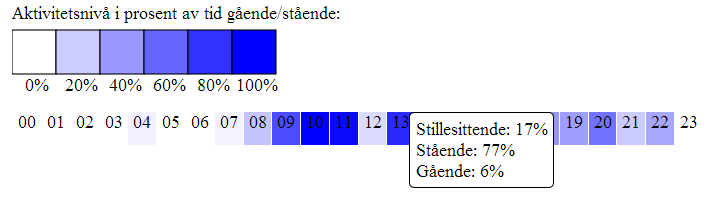
\includegraphics[width=\textwidth]{t1FirstSingle.png}
    \caption{T1 day.}
  \end{subfigure}
  \begin{subfigure}[b]{0.45\textwidth}
    \centering
    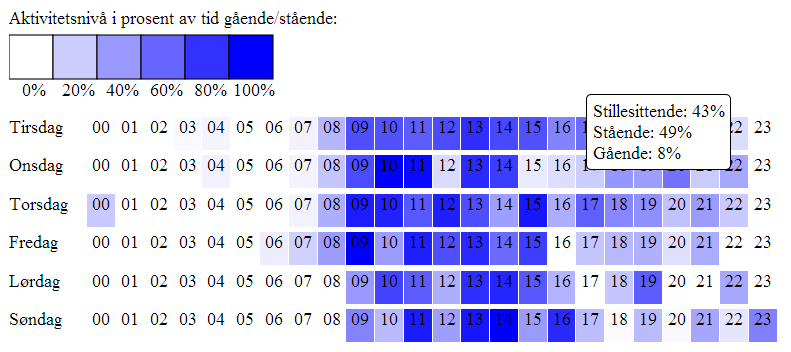
\includegraphics[width=\textwidth]{t1FirstWeek.png}
    \caption{T1 week.}
  \end{subfigure}
  \\
  \begin{subfigure}[b]{0.45\textwidth}
    \centering
    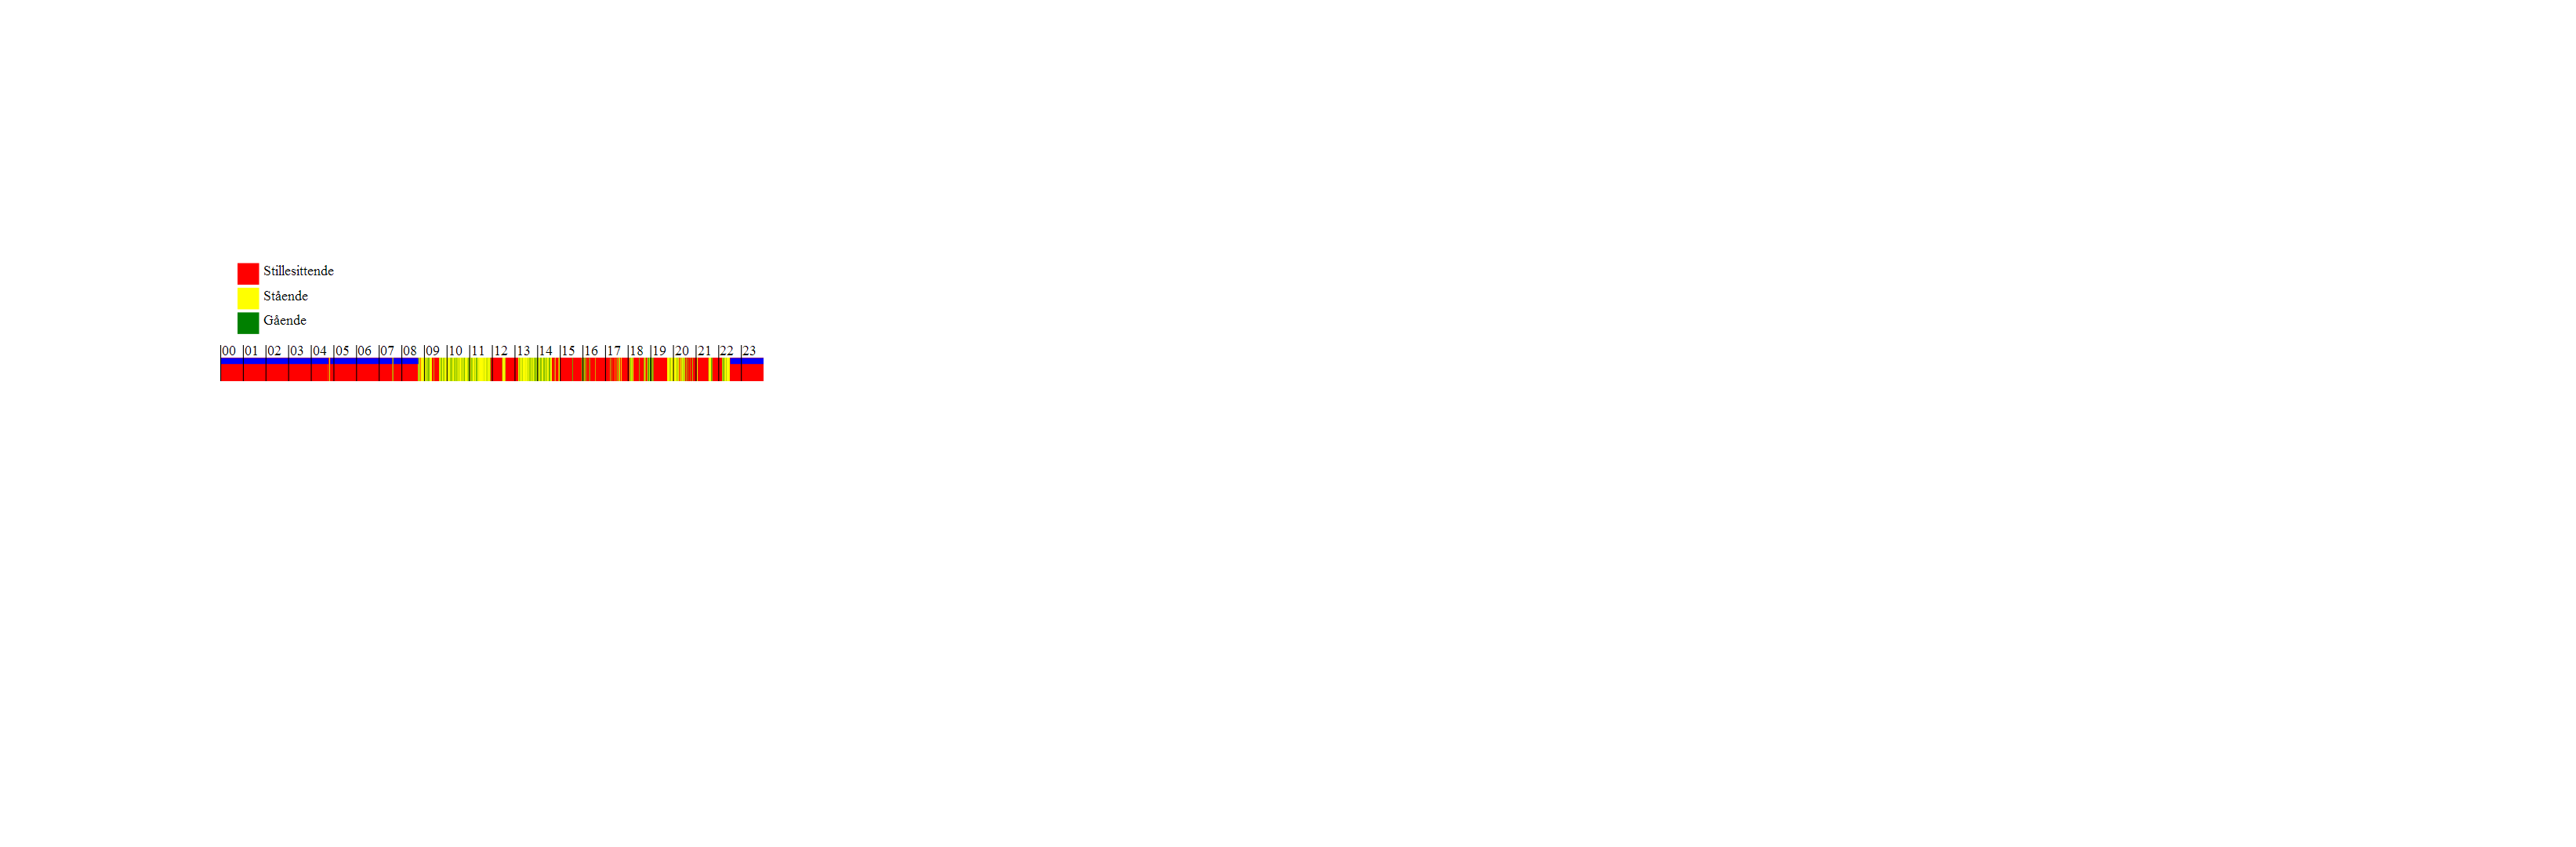
\includegraphics[width=\textwidth]{t2FirstSingle.png}
    \caption{T2 day.}
  \end{subfigure}
  \begin{subfigure}[b]{0.45\textwidth}
    \centering
    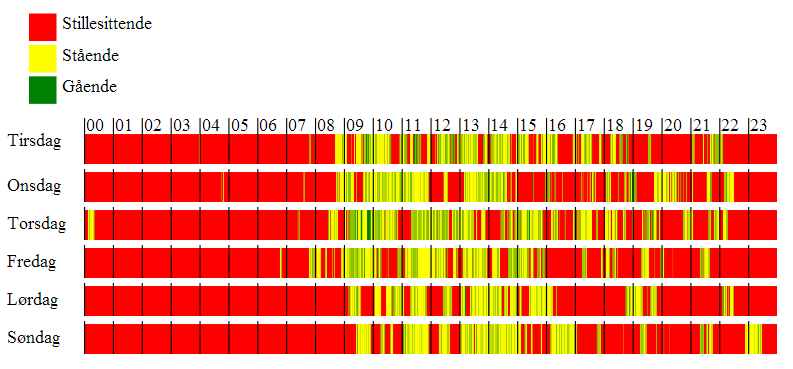
\includegraphics[width=\textwidth]{t2FirstWeek.png}
    \caption{T2 week.}
  \end{subfigure}
  \\
  \begin{subfigure}[b]{0.45\textwidth}
    \centering
    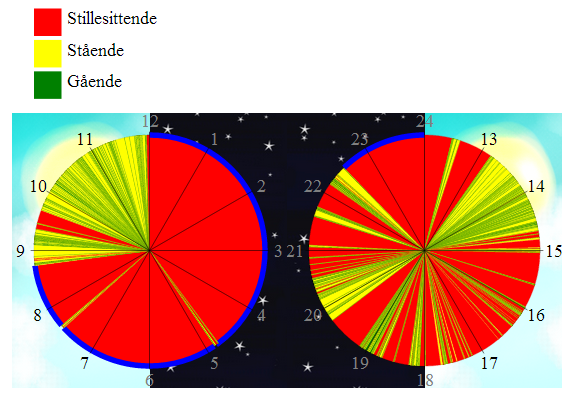
\includegraphics[width=\textwidth]{t3First.png}
    \caption{T3 with highlighting}
  \end{subfigure}
  \begin{subfigure}[b]{0.45\textwidth}
    \centering
    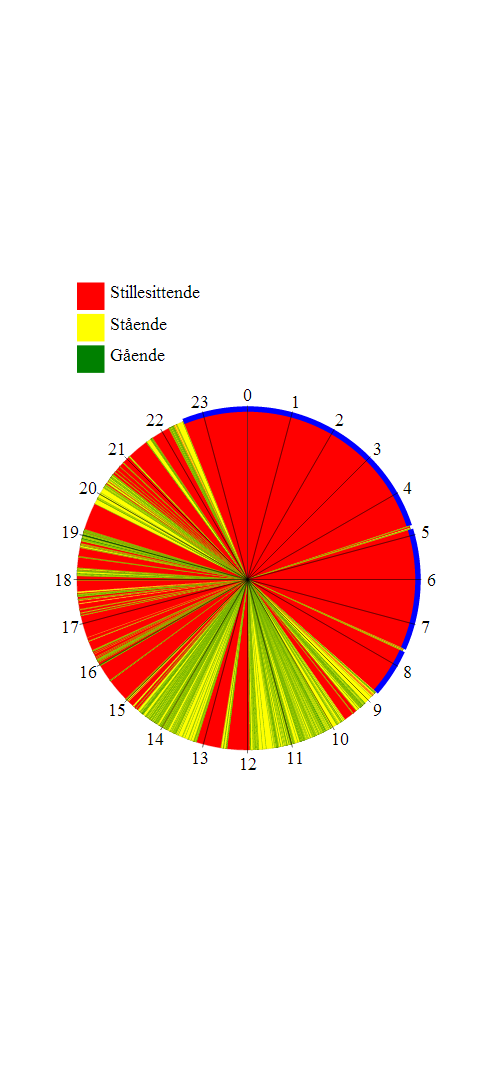
\includegraphics[width=\textwidth]{t4First.png}
    \caption{T4 with highlighting}
  \end{subfigure}
  \caption{Timeline charts.}
  \label{fig:tFirst}
\end{figure}  
